\documentclass[]{article}
\usepackage{lmodern}
\usepackage{amssymb,amsmath}
\usepackage{ifxetex,ifluatex}
\usepackage{fixltx2e} % provides \textsubscript
\ifnum 0\ifxetex 1\fi\ifluatex 1\fi=0 % if pdftex
  \usepackage[T1]{fontenc}
  \usepackage[utf8]{inputenc}
\else % if luatex or xelatex
  \ifxetex
    \usepackage{mathspec}
  \else
    \usepackage{fontspec}
  \fi
  \defaultfontfeatures{Ligatures=TeX,Scale=MatchLowercase}
\fi
% use upquote if available, for straight quotes in verbatim environments
\IfFileExists{upquote.sty}{\usepackage{upquote}}{}
% use microtype if available
\IfFileExists{microtype.sty}{%
\usepackage{microtype}
\UseMicrotypeSet[protrusion]{basicmath} % disable protrusion for tt fonts
}{}
\usepackage[margin=1in]{geometry}
\usepackage{hyperref}
\hypersetup{unicode=true,
            pdftitle={Latent TB infection (LTBI) Bayesian multiparameter evidence synthesis (MPES)},
            pdfauthor={Nathan Green (Imperial College London)},
            pdfborder={0 0 0},
            breaklinks=true}
\urlstyle{same}  % don't use monospace font for urls
\usepackage{color}
\usepackage{fancyvrb}
\newcommand{\VerbBar}{|}
\newcommand{\VERB}{\Verb[commandchars=\\\{\}]}
\DefineVerbatimEnvironment{Highlighting}{Verbatim}{commandchars=\\\{\}}
% Add ',fontsize=\small' for more characters per line
\usepackage{framed}
\definecolor{shadecolor}{RGB}{248,248,248}
\newenvironment{Shaded}{\begin{snugshade}}{\end{snugshade}}
\newcommand{\AlertTok}[1]{\textcolor[rgb]{0.94,0.16,0.16}{#1}}
\newcommand{\AnnotationTok}[1]{\textcolor[rgb]{0.56,0.35,0.01}{\textbf{\textit{#1}}}}
\newcommand{\AttributeTok}[1]{\textcolor[rgb]{0.77,0.63,0.00}{#1}}
\newcommand{\BaseNTok}[1]{\textcolor[rgb]{0.00,0.00,0.81}{#1}}
\newcommand{\BuiltInTok}[1]{#1}
\newcommand{\CharTok}[1]{\textcolor[rgb]{0.31,0.60,0.02}{#1}}
\newcommand{\CommentTok}[1]{\textcolor[rgb]{0.56,0.35,0.01}{\textit{#1}}}
\newcommand{\CommentVarTok}[1]{\textcolor[rgb]{0.56,0.35,0.01}{\textbf{\textit{#1}}}}
\newcommand{\ConstantTok}[1]{\textcolor[rgb]{0.00,0.00,0.00}{#1}}
\newcommand{\ControlFlowTok}[1]{\textcolor[rgb]{0.13,0.29,0.53}{\textbf{#1}}}
\newcommand{\DataTypeTok}[1]{\textcolor[rgb]{0.13,0.29,0.53}{#1}}
\newcommand{\DecValTok}[1]{\textcolor[rgb]{0.00,0.00,0.81}{#1}}
\newcommand{\DocumentationTok}[1]{\textcolor[rgb]{0.56,0.35,0.01}{\textbf{\textit{#1}}}}
\newcommand{\ErrorTok}[1]{\textcolor[rgb]{0.64,0.00,0.00}{\textbf{#1}}}
\newcommand{\ExtensionTok}[1]{#1}
\newcommand{\FloatTok}[1]{\textcolor[rgb]{0.00,0.00,0.81}{#1}}
\newcommand{\FunctionTok}[1]{\textcolor[rgb]{0.00,0.00,0.00}{#1}}
\newcommand{\ImportTok}[1]{#1}
\newcommand{\InformationTok}[1]{\textcolor[rgb]{0.56,0.35,0.01}{\textbf{\textit{#1}}}}
\newcommand{\KeywordTok}[1]{\textcolor[rgb]{0.13,0.29,0.53}{\textbf{#1}}}
\newcommand{\NormalTok}[1]{#1}
\newcommand{\OperatorTok}[1]{\textcolor[rgb]{0.81,0.36,0.00}{\textbf{#1}}}
\newcommand{\OtherTok}[1]{\textcolor[rgb]{0.56,0.35,0.01}{#1}}
\newcommand{\PreprocessorTok}[1]{\textcolor[rgb]{0.56,0.35,0.01}{\textit{#1}}}
\newcommand{\RegionMarkerTok}[1]{#1}
\newcommand{\SpecialCharTok}[1]{\textcolor[rgb]{0.00,0.00,0.00}{#1}}
\newcommand{\SpecialStringTok}[1]{\textcolor[rgb]{0.31,0.60,0.02}{#1}}
\newcommand{\StringTok}[1]{\textcolor[rgb]{0.31,0.60,0.02}{#1}}
\newcommand{\VariableTok}[1]{\textcolor[rgb]{0.00,0.00,0.00}{#1}}
\newcommand{\VerbatimStringTok}[1]{\textcolor[rgb]{0.31,0.60,0.02}{#1}}
\newcommand{\WarningTok}[1]{\textcolor[rgb]{0.56,0.35,0.01}{\textbf{\textit{#1}}}}
\usepackage{graphicx,grffile}
\makeatletter
\def\maxwidth{\ifdim\Gin@nat@width>\linewidth\linewidth\else\Gin@nat@width\fi}
\def\maxheight{\ifdim\Gin@nat@height>\textheight\textheight\else\Gin@nat@height\fi}
\makeatother
% Scale images if necessary, so that they will not overflow the page
% margins by default, and it is still possible to overwrite the defaults
% using explicit options in \includegraphics[width, height, ...]{}
\setkeys{Gin}{width=\maxwidth,height=\maxheight,keepaspectratio}
\IfFileExists{parskip.sty}{%
\usepackage{parskip}
}{% else
\setlength{\parindent}{0pt}
\setlength{\parskip}{6pt plus 2pt minus 1pt}
}
\setlength{\emergencystretch}{3em}  % prevent overfull lines
\providecommand{\tightlist}{%
  \setlength{\itemsep}{0pt}\setlength{\parskip}{0pt}}
\setcounter{secnumdepth}{0}
% Redefines (sub)paragraphs to behave more like sections
\ifx\paragraph\undefined\else
\let\oldparagraph\paragraph
\renewcommand{\paragraph}[1]{\oldparagraph{#1}\mbox{}}
\fi
\ifx\subparagraph\undefined\else
\let\oldsubparagraph\subparagraph
\renewcommand{\subparagraph}[1]{\oldsubparagraph{#1}\mbox{}}
\fi

%%% Use protect on footnotes to avoid problems with footnotes in titles
\let\rmarkdownfootnote\footnote%
\def\footnote{\protect\rmarkdownfootnote}

%%% Change title format to be more compact
\usepackage{titling}

% Create subtitle command for use in maketitle
\providecommand{\subtitle}[1]{
  \posttitle{
    \begin{center}\large#1\end{center}
    }
}

\setlength{\droptitle}{-2em}

  \title{Latent TB infection (LTBI) Bayesian multiparameter evidence synthesis
(MPES)}
    \pretitle{\vspace{\droptitle}\centering\huge}
  \posttitle{\par}
    \author{Nathan Green (Imperial College London)}
    \preauthor{\centering\large\emph}
  \postauthor{\par}
      \predate{\centering\large\emph}
  \postdate{\par}
    \date{26/11/2019}


\begin{document}
\maketitle

\hypertarget{introduction}{%
\subsubsection{Introduction}\label{introduction}}

We have several data sources which can inform the estimation of LTBI
prevalence in subpopulations. We will formulate a Bayesian evidence
synthesis model to do this.

\hypertarget{model-with-screening-and-progression-count-data-e.g.-predict}{%
\subsubsection{Model with screening and progression count data
(e.g.~PREDICT)}\label{model-with-screening-and-progression-count-data-e.g.-predict}}

Define a group to be a combination of multiple values across covariates.
For example, a 16 to 18 years old, white British male. We will fit
separate models to each group in the following. A regression model with
group covariates could be developed. We assume that the LTBI test
sensitivity and specificity is the same for all groups. We also assume
that the probability of progressing to active TB is the same for all
groups. For \(N\) groups the model formulae are

\begin{eqnarray*}
X_l(j) &\sim& Bin(X_m(j), p_l(j))\\
p_{+}(j) &=& p_l(j) \times sens + (1-p_l(j)) \times (1-spec)\\
X_p(j) &\sim& Bin(X_m(j), p_+(j))\\
X_{TB}(j) &\sim& Bin(X_l(j), \lambda)
\end{eqnarray*}

where \(j\) is the group index, \(X_l\) is the (unobserved) number of
LTBI individuals, \(X_m\) is the observed number of migrants i.e.~the
total sample, \(X_p\) is the observed number of positive tests in the
migrant population, \(X_{TB}\) is the observed number of active TB
cases, \(p_l\) is the probability of having LTBI i.e.~prevalence,
\(p_+\) is the test positivity, \(\lambda\) is the proportion of LTBI
individuals who progress to active TB (in the total time at risk),
\(sens\) is the test sensitivity, \(spec\) is the test specificity.

The Directed Acyclic Graph (DAG) for this model is given below.

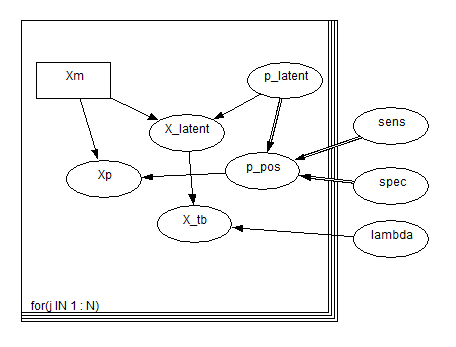
\includegraphics{DAG-time-independent.PNG}

The main model BUGS code is given below.

\begin{Shaded}
\begin{Highlighting}[]
\CommentTok{## LTBI screening evidence synthesis model ----}

\NormalTok{model \{}

  \ControlFlowTok{for}\NormalTok{ (j }\ControlFlowTok{in} \DecValTok{1}\OperatorTok{:}\NormalTok{len_gp) \{}

\NormalTok{      X_latent[j] }\OperatorTok{~}\StringTok{ }\KeywordTok{dbin}\NormalTok{(p_latent[j], Xm[j])}
\NormalTok{      p_pos[j] <-}\StringTok{ }\NormalTok{(p_latent[j]}\OperatorTok{*}\NormalTok{sens) }\OperatorTok{+}\StringTok{ }\NormalTok{(}\DecValTok{1} \OperatorTok{-}\StringTok{ }\NormalTok{p_latent[j])}\OperatorTok{*}\NormalTok{(}\DecValTok{1} \OperatorTok{-}\StringTok{ }\NormalTok{spec)}
\NormalTok{      Xp[j] }\OperatorTok{~}\StringTok{ }\KeywordTok{dbin}\NormalTok{(p_pos[j], Xm[j])}
\NormalTok{      Xtb[j] }\OperatorTok{~}\StringTok{ }\KeywordTok{dbin}\NormalTok{(lambda, X_latent[j])}
\NormalTok{    \}}
\NormalTok{\}}
\end{Highlighting}
\end{Shaded}

\hypertarget{prior-distributions}{%
\paragraph{Prior distributions}\label{prior-distributions}}

Vague prior were used in the first instance. When fitting to the actual
real-life data we will have informative priors for the test performance,
progression rates and prevalence within groups from previous studies.

\begin{eqnarray*}
sens &\sim& Beta(a_{sens}, b_{sens})\\
sens &\sim& Beta(a_{spec}, b_{spec})\\
\lambda &\sim& Beta(a_{\lambda}, b_{\lambda})\\
logit(p_l) &\sim& Normal(0, \sigma^2_l) 
\end{eqnarray*}

The corresponding BUGS code is given below.

\begin{Shaded}
\begin{Highlighting}[]
\NormalTok{sens }\OperatorTok{~}\StringTok{ }\KeywordTok{dbeta}\NormalTok{(}\DecValTok{100}\NormalTok{, }\DecValTok{5}\NormalTok{)   }\CommentTok{# mean 0.96}
\NormalTok{spec }\OperatorTok{~}\StringTok{ }\KeywordTok{dbeta}\NormalTok{(}\DecValTok{100}\NormalTok{, }\DecValTok{5}\NormalTok{)   }\CommentTok{# mean 0.96}
\NormalTok{lambda }\OperatorTok{~}\StringTok{ }\KeywordTok{dbeta}\NormalTok{(}\DecValTok{5}\NormalTok{, }\DecValTok{100}\NormalTok{) }\CommentTok{# mean 0.05}

\CommentTok{# this is not a robust prior}
\ControlFlowTok{for}\NormalTok{ (j }\ControlFlowTok{in} \DecValTok{1}\OperatorTok{:}\NormalTok{len_gp) \{}
\NormalTok{  logitp_latent[j] }\OperatorTok{~}\StringTok{ }\KeywordTok{dnorm}\NormalTok{(}\DecValTok{0}\NormalTok{, }\FloatTok{0.001}\NormalTok{)}
\NormalTok{  p_latent[j] <-}\StringTok{ }\KeywordTok{exp}\NormalTok{(logitp_latent[j]) }\OperatorTok{/}\StringTok{ }\NormalTok{(}\DecValTok{1} \OperatorTok{+}\StringTok{ }\KeywordTok{exp}\NormalTok{(logitp_latent[j]))}
\NormalTok{\}}
\end{Highlighting}
\end{Shaded}

\hypertarget{running-the-winbugs-model-from-r}{%
\subsubsection{Running the WinBUGS model from
R}\label{running-the-winbugs-model-from-r}}

For simplicity, we demonstrate the model on dummy data. We have two
groups \(j = 1, 2\).

\begin{Shaded}
\begin{Highlighting}[]
\KeywordTok{library}\NormalTok{(R2jags)}
\KeywordTok{library}\NormalTok{(R2WinBUGS)}
\KeywordTok{library}\NormalTok{(purrr)}
\end{Highlighting}
\end{Shaded}

\begin{Shaded}
\begin{Highlighting}[]
\NormalTok{dat <-}\StringTok{ }\KeywordTok{read.csv}\NormalTok{(here}\OperatorTok{::}\KeywordTok{here}\NormalTok{(}\StringTok{"data input"}\NormalTok{, }\StringTok{"PREDICT_dummy.csv"}\NormalTok{), }\DataTypeTok{header =} \OtherTok{TRUE}\NormalTok{)}

\NormalTok{jags_dat_input <-}
\StringTok{  }\KeywordTok{list}\NormalTok{(}
    \DataTypeTok{len_gp =} \KeywordTok{nrow}\NormalTok{(dat),                   }\CommentTok{# number of groups}
    \DataTypeTok{Xm  =}\NormalTok{ dat}\OperatorTok{$}\NormalTok{n_migrant,                  }\CommentTok{# number of migrants}
    \DataTypeTok{Xp  =}\NormalTok{ dat}\OperatorTok{$}\NormalTok{n_pos,                      }\CommentTok{# number of positive test results}
    \DataTypeTok{Xtb =}\NormalTok{ dat}\OperatorTok{$}\NormalTok{n_tb                        }\CommentTok{# number of observed active tb cases}
\NormalTok{  )}

\NormalTok{jags_dat_input}
\end{Highlighting}
\end{Shaded}

\begin{verbatim}
## $len_gp
## [1] 2
## 
## $Xm
## [1] 1000  500
## 
## $Xp
## [1] 300 250
## 
## $Xtb
## [1] 30 10
\end{verbatim}

\begin{Shaded}
\begin{Highlighting}[]
\NormalTok{params <-}
\StringTok{  }\KeywordTok{c}\NormalTok{(}\StringTok{"sens"}\NormalTok{, }\StringTok{"spec"}\NormalTok{,}
    \StringTok{"lambda"}\NormalTok{,}
    \StringTok{"p_latent"}
\NormalTok{  )}

\NormalTok{n_iter <-}\StringTok{ }\FloatTok{1e6}
\NormalTok{n_burnin <-}\StringTok{ }\FloatTok{1e3}
\NormalTok{n_thin <-}\StringTok{ }\FloatTok{1e2} \CommentTok{#floor((n_iter - n_burnin)/500)}
\end{Highlighting}
\end{Shaded}

Finally, run the MCMC. We specify 2 chains, a burn-in period, thinning
rate and which parameters to monitor.

\begin{Shaded}
\begin{Highlighting}[]
\NormalTok{out <-}\StringTok{ }\KeywordTok{jags}\NormalTok{(jags_dat_input,}
            \DataTypeTok{parameters.to.save =}\NormalTok{ params,}
            \DataTypeTok{model.file =}\NormalTok{ here}\OperatorTok{::}\KeywordTok{here}\NormalTok{(}\StringTok{"scripts"}\NormalTok{, }\StringTok{"BUGS_code_Xl_distn.txt"}\NormalTok{),}
            \DataTypeTok{n.chains =} \DecValTok{2}\NormalTok{,}
            \DataTypeTok{n.iter =}\NormalTok{ n_iter,}
            \DataTypeTok{n.burnin =}\NormalTok{ n_burnin,}
            \DataTypeTok{n.thin =}\NormalTok{ n_thin,}
            \DataTypeTok{DIC =} \OtherTok{TRUE}\NormalTok{,}
            \DataTypeTok{working.directory =}\NormalTok{ here}\OperatorTok{::}\KeywordTok{here}\NormalTok{(}\StringTok{"scripts"}\NormalTok{),}
            \DataTypeTok{progress.bar =} \StringTok{"text"}\NormalTok{)}
\end{Highlighting}
\end{Shaded}

\hypertarget{evaluate-output}{%
\subsubsection{Evaluate output}\label{evaluate-output}}

We will use the plotting functions from the
\href{https://cran.r-project.org/web/packages/MCMCvis/vignettes/MCMCvis.html}{\texttt{MCMCvis}}
package. The priors are the red lines.

\begin{Shaded}
\begin{Highlighting}[]
\KeywordTok{library}\NormalTok{(MCMCvis)}

\NormalTok{n_sample <-}\StringTok{ }\NormalTok{(n_iter}\OperatorTok{-}\NormalTok{n_burnin)}\OperatorTok{/}\NormalTok{n_thin}

\CommentTok{## sample from priors ----}

\NormalTok{sens <-}\StringTok{ }\KeywordTok{rbeta}\NormalTok{(}\DataTypeTok{n =}\NormalTok{ n_sample, }\DataTypeTok{shape1 =} \DecValTok{100}\NormalTok{, }\DataTypeTok{shape2 =} \DecValTok{5}\NormalTok{)}
\NormalTok{spec <-}\StringTok{ }\KeywordTok{rbeta}\NormalTok{(}\DataTypeTok{n =}\NormalTok{ n_sample, }\DataTypeTok{shape1 =} \DecValTok{100}\NormalTok{, }\DataTypeTok{shape2 =} \DecValTok{5}\NormalTok{)}
\NormalTok{lambda <-}\StringTok{ }\KeywordTok{rbeta}\NormalTok{(}\DataTypeTok{n =}\NormalTok{ n_sample, }\DataTypeTok{shape1 =} \DecValTok{5}\NormalTok{, }\DataTypeTok{shape2 =} \DecValTok{100}\NormalTok{)}
\NormalTok{logitp_latent <-}\StringTok{ }\KeywordTok{rnorm}\NormalTok{(}\DataTypeTok{n =}\NormalTok{ n_sample, }\DataTypeTok{mean =} \DecValTok{0}\NormalTok{, }\DataTypeTok{sd =} \DecValTok{1}\OperatorTok{/}\FloatTok{0.001}\NormalTok{)}
\NormalTok{p_latent <-}\StringTok{ }\KeywordTok{exp}\NormalTok{(logitp_latent) }\OperatorTok{/}\StringTok{ }\NormalTok{(}\DecValTok{1} \OperatorTok{+}\StringTok{ }\KeywordTok{exp}\NormalTok{(logitp_latent))}
\NormalTok{p_latent[}\KeywordTok{is.nan}\NormalTok{(p_latent)] <-}\StringTok{ }\DecValTok{0} \CommentTok{#remove NaN}
\end{Highlighting}
\end{Shaded}

Trace plots and prior-posterior density plots are shown below.

\begin{Shaded}
\begin{Highlighting}[]
\KeywordTok{MCMCtrace}\NormalTok{(out,}
          \DataTypeTok{pdf =} \OtherTok{FALSE}\NormalTok{,}
          \DataTypeTok{ind =} \OtherTok{TRUE}\NormalTok{,}
          \DataTypeTok{iter =}\NormalTok{ n_sample,}
          \DataTypeTok{params =} \KeywordTok{c}\NormalTok{(}\StringTok{"lambda"}\NormalTok{, }\StringTok{"sens"}\NormalTok{, }\StringTok{"spec"}\NormalTok{, }\StringTok{"p_latent"}\NormalTok{),}
          \DataTypeTok{priors =} \KeywordTok{as.matrix}\NormalTok{(}\KeywordTok{data.frame}\NormalTok{(lambda, sens, spec, p_latent, p_latent)))}
\end{Highlighting}
\end{Shaded}

\includegraphics{evid-synthesis_files/figure-latex/unnamed-chunk-5-1.pdf}
\includegraphics{evid-synthesis_files/figure-latex/unnamed-chunk-5-2.pdf}

A posterior forest plot is shown below.

\begin{Shaded}
\begin{Highlighting}[]
\KeywordTok{MCMCplot}\NormalTok{(out,}
         \DataTypeTok{params =} \KeywordTok{c}\NormalTok{(}\StringTok{"sens"}\NormalTok{, }\StringTok{"spec"}\NormalTok{, }\StringTok{"lambda"}\NormalTok{, }\StringTok{"p_latent"}\NormalTok{))}
\end{Highlighting}
\end{Shaded}

\includegraphics{evid-synthesis_files/figure-latex/unnamed-chunk-6-1.pdf}

Using the \texttt{coda} package, BGR plots are show below.

\begin{Shaded}
\begin{Highlighting}[]
\NormalTok{coda}\OperatorTok{::}\KeywordTok{gelman.plot}\NormalTok{(mcmcplots}\OperatorTok{::}\KeywordTok{as.mcmc.rjags}\NormalTok{(out), }\DataTypeTok{cex =} \DecValTok{2}\NormalTok{, }\DataTypeTok{cex.main =} \DecValTok{3}\NormalTok{)}
\end{Highlighting}
\end{Shaded}

\includegraphics{evid-synthesis_files/figure-latex/unnamed-chunk-7-1.pdf}

\hypertarget{functional-x_l}{%
\paragraph{\texorpdfstring{Functional
\(X_l\)}{Functional X\_l}}\label{functional-x_l}}

The estimate for \(X_l\) is made as a likelihood in the above model. It
may make more sense to have it as a functional relationship of migrant
populations and probability of LTBI, since estimating \(p_l\) and
\(X_l\) is unobserved. This has the problem that it must be an integer
value to then be used in the Binomial distribution. One solution is
simply to round down the product, giving

\begin{eqnarray*}
X_l(j) &=& \lfloor X_m(j) \times p_l(j) \rfloor
\end{eqnarray*}

The remaining model is exactly the same as above. The output is given
below.

\includegraphics{evid-synthesis_files/figure-latex/unnamed-chunk-9-1.pdf}
\includegraphics{evid-synthesis_files/figure-latex/unnamed-chunk-9-2.pdf}

\includegraphics{evid-synthesis_files/figure-latex/unnamed-chunk-10-1.pdf}

\includegraphics{evid-synthesis_files/figure-latex/unnamed-chunk-11-1.pdf}

\hypertarget{model-with-progression-data-only-e.g.-pes-ets}{%
\subsubsection{Model with progression data only
(e.g.~PES-ETS)}\label{model-with-progression-data-only-e.g.-pes-ets}}

Now assume that we do not observe the LTBI positivity of a cohort of
individuals followed-up over time. We parameterise the model so that the
probability of active TB is the product of LTBI infection and
progression. Using the same notation as above, the new formula is

\begin{eqnarray*}
X_{TB}(j) &\sim& Bin(X_m(j), p_l(j) \times \lambda)
\end{eqnarray*}

The DAG for this model is given below.

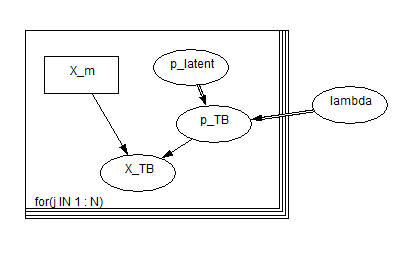
\includegraphics{DAG-ETS.PNG}

The BUGS code is as follows.

\begin{Shaded}
\begin{Highlighting}[]
\NormalTok{model \{}

  \ControlFlowTok{for}\NormalTok{ (j }\ControlFlowTok{in} \DecValTok{1}\OperatorTok{:}\NormalTok{len_gp) \{}

\NormalTok{      Xtb[j] }\OperatorTok{~}\StringTok{ }\KeywordTok{dbin}\NormalTok{(p_TB[j], Xm[j])}
\NormalTok{      p_TB[j] <-}\StringTok{ }\NormalTok{lambda}\OperatorTok{*}\NormalTok{p_latent[j]}
\NormalTok{    \}}
\NormalTok{\}}
\end{Highlighting}
\end{Shaded}

with the same priors on \(\lambda\) and \(p_l\) as before. For
exposition, we will use the same data as before but now we do not
observe the test results. This therefore gives the following inputs.

\begin{Shaded}
\begin{Highlighting}[]
\NormalTok{jags_dat_input <-}
\StringTok{  }\KeywordTok{list}\NormalTok{(}
    \DataTypeTok{len_gp =} \KeywordTok{nrow}\NormalTok{(dat),}
    \DataTypeTok{Xm  =}\NormalTok{ dat}\OperatorTok{$}\NormalTok{n_migrant,}
    \DataTypeTok{Xtb =}\NormalTok{ dat}\OperatorTok{$}\NormalTok{n_tb}
\NormalTok{  )}

\NormalTok{params <-}
\StringTok{  }\KeywordTok{c}\NormalTok{(}\StringTok{"lambda"}\NormalTok{,}
    \StringTok{"p_latent"}\NormalTok{)}
\end{Highlighting}
\end{Shaded}

The output is given below.

\includegraphics{evid-synthesis_files/figure-latex/unnamed-chunk-14-1.pdf}

\includegraphics{evid-synthesis_files/figure-latex/unnamed-chunk-15-1.pdf}

\includegraphics{evid-synthesis_files/figure-latex/unnamed-chunk-16-1.pdf}

\hypertarget{evidence-synthesis-model-e.g.-predict-and-pes-ets}{%
\subsubsection{Evidence synthesis model (e.g.~PREDICT and
PES-ETS)}\label{evidence-synthesis-model-e.g.-predict-and-pes-ets}}

We can now combine the two separate models to create a single model
which uses both data sources simultaneously.

The DAG for the model with \(X_l\) sampled is given below.

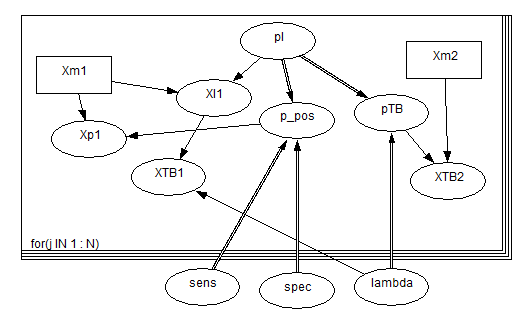
\includegraphics{DAG-full_model.PNG}

The DAG for a deterministic functional form is

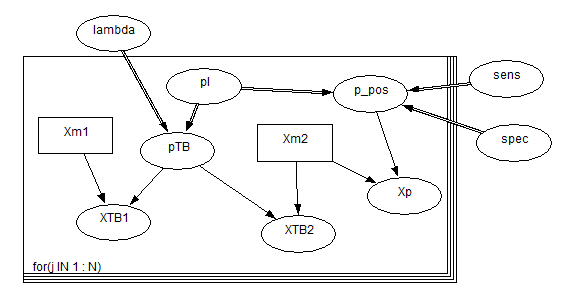
\includegraphics{DAG-full_model_pTB.PNG}

\hypertarget{datasets-in-agreement}{%
\paragraph{Datasets in agreement}\label{datasets-in-agreement}}

First, create the input data variable, where there are now two rows in
\(X_m\) and \(X_{tb}\) corresponding to different datasets.

\begin{Shaded}
\begin{Highlighting}[]
\NormalTok{jags_dat_input <-}
\StringTok{  }\KeywordTok{list}\NormalTok{(}
    \DataTypeTok{len_gp =} \KeywordTok{nrow}\NormalTok{(dat),             }\CommentTok{# number of groups}
    \DataTypeTok{Xm  =} \KeywordTok{rbind}\NormalTok{(dat}\OperatorTok{$}\NormalTok{n_migrant,}
\NormalTok{                dat}\OperatorTok{$}\NormalTok{n_migrant),     }\CommentTok{# number of migrants}
    \DataTypeTok{Xp  =}\NormalTok{ dat}\OperatorTok{$}\NormalTok{n_pos,                }\CommentTok{# number of positive test results}
    \DataTypeTok{Xtb =} \KeywordTok{rbind}\NormalTok{(dat}\OperatorTok{$}\NormalTok{n_tb,}
\NormalTok{                dat}\OperatorTok{$}\NormalTok{n_tb)           }\CommentTok{# number of observed active tb cases}
\NormalTok{  )}

\NormalTok{jags_dat_input}
\end{Highlighting}
\end{Shaded}

\begin{verbatim}
## $len_gp
## [1] 2
## 
## $Xm
##      [,1] [,2]
## [1,] 1000  500
## [2,] 1000  500
## 
## $Xp
## [1] 300 250
## 
## $Xtb
##      [,1] [,2]
## [1,]   30   10
## [2,]   30   10
\end{verbatim}

\begin{Shaded}
\begin{Highlighting}[]
\NormalTok{params <-}
\StringTok{  }\KeywordTok{c}\NormalTok{(}\StringTok{"sens"}\NormalTok{, }\StringTok{"spec"}\NormalTok{,}
    \StringTok{"lambda"}\NormalTok{,}
    \StringTok{"p_latent"}
\NormalTok{  )}
\end{Highlighting}
\end{Shaded}

\begin{Shaded}
\begin{Highlighting}[]
\NormalTok{out <-}\StringTok{ }\KeywordTok{jags}\NormalTok{(jags_dat_input,}
            \DataTypeTok{parameters.to.save =}\NormalTok{ params,}
            \DataTypeTok{model.file =}\NormalTok{ here}\OperatorTok{::}\KeywordTok{here}\NormalTok{(}\StringTok{"scripts"}\NormalTok{, }\StringTok{"BUGS_code_full_Xl_fn.txt"}\NormalTok{),}
            \DataTypeTok{n.chains =} \DecValTok{2}\NormalTok{,}
            \DataTypeTok{n.iter =}\NormalTok{ n_iter,}
            \DataTypeTok{n.burnin =}\NormalTok{ n_burnin,}
            \DataTypeTok{n.thin =}\NormalTok{ n_thin,}
            \DataTypeTok{DIC =} \OtherTok{TRUE}\NormalTok{,}
            \DataTypeTok{working.directory =}\NormalTok{ here}\OperatorTok{::}\KeywordTok{here}\NormalTok{(}\StringTok{"scripts"}\NormalTok{),}
            \DataTypeTok{progress.bar =} \StringTok{"text"}\NormalTok{)}
\end{Highlighting}
\end{Shaded}

The output is given below.

\includegraphics{evid-synthesis_files/figure-latex/unnamed-chunk-19-1.pdf}
\includegraphics{evid-synthesis_files/figure-latex/unnamed-chunk-19-2.pdf}

\includegraphics{evid-synthesis_files/figure-latex/unnamed-chunk-20-1.pdf}

\includegraphics{evid-synthesis_files/figure-latex/unnamed-chunk-21-1.pdf}

\hypertarget{datasets-in-conflict}{%
\paragraph{Datasets in conflict}\label{datasets-in-conflict}}

Now suppose that the two data source do not agree with each other.

\begin{Shaded}
\begin{Highlighting}[]
\NormalTok{jags_dat_input}\OperatorTok{$}\NormalTok{Xtb[}\DecValTok{2}\NormalTok{, ] <-}\StringTok{ }\KeywordTok{c}\NormalTok{(}\DecValTok{100}\NormalTok{, }\DecValTok{5}\NormalTok{) }\CommentTok{# vs c(30, 10)}
\end{Highlighting}
\end{Shaded}

\begin{Shaded}
\begin{Highlighting}[]
\NormalTok{out <-}\StringTok{ }\KeywordTok{jags}\NormalTok{(jags_dat_input,}
            \DataTypeTok{parameters.to.save =}\NormalTok{ params,}
            \DataTypeTok{model.file =}\NormalTok{ here}\OperatorTok{::}\KeywordTok{here}\NormalTok{(}\StringTok{"scripts"}\NormalTok{, }\StringTok{"BUGS_code_full_Xl_fn.txt"}\NormalTok{),}
            \DataTypeTok{n.chains =} \DecValTok{2}\NormalTok{,}
            \DataTypeTok{n.iter =}\NormalTok{ n_iter,}
            \DataTypeTok{n.burnin =}\NormalTok{ n_burnin,}
            \DataTypeTok{n.thin =}\NormalTok{ n_thin,}
            \DataTypeTok{DIC =} \OtherTok{TRUE}\NormalTok{,}
            \DataTypeTok{working.directory =}\NormalTok{ here}\OperatorTok{::}\KeywordTok{here}\NormalTok{(}\StringTok{"scripts"}\NormalTok{),}
            \DataTypeTok{progress.bar =} \StringTok{"text"}\NormalTok{)}
\end{Highlighting}
\end{Shaded}

The output is given below.

\includegraphics{evid-synthesis_files/figure-latex/unnamed-chunk-24-1.pdf}
\includegraphics{evid-synthesis_files/figure-latex/unnamed-chunk-24-2.pdf}

\includegraphics{evid-synthesis_files/figure-latex/unnamed-chunk-25-1.pdf}

\includegraphics{evid-synthesis_files/figure-latex/unnamed-chunk-26-1.pdf}

\hypertarget{ltbi-prevalence-regression-model}{%
\paragraph{LTBI prevalence regression
model}\label{ltbi-prevalence-regression-model}}

Rather than have a stratified model with a prior on the probability of
latent TB, \(p_l\), we can have a regression model with priors on the
coefficients of a fixed-effects linear equation.

\[
logit(p_l) = \beta_0 + \beta_1 sex + \beta_{21} ethn_1 + \beta_{22} ethn_2 + \cdots + \beta_{31} agegrp_1 + \beta_{32} agrgrp_2 + \cdots
\]

This now also allows us to estimate expected prevalence for unobserved
categories.


\end{document}
